\documentclass[24pt, a4paper, portrait]{article}

\usepackage[utf8]{inputenc}
\usepackage[a4paper,left=2cm,right=2cm,top=1cm,bottom=2cm]{geometry}
\usepackage{graphicx}
\usepackage{array}

\graphicspath{{./img/}}

\begin{document}

\pagestyle{empty}

\raggedleft


\includegraphics[width=0.4\textwidth]{logo}

\vspace{1cm}
\sffamily
\centering
\huge

\textbf{Vor Verlassen des Labors bitte auschecken!}

\vspace{1cm}

\raggedright
\Large

Um bei einem Covid-19-Fall in einem unserer Labore mögliche Infektionsketten zurückverfolgen zu können, müssen Beginn und Ende des Aufenthalts im Labor festgehalten werden.

\medskip

Scannen Sie dazu den folgenden QR-Code oder folgen Sie diesem Link: \textbf{wiki.mi.ur.de/lab/checkout}

\medskip

Füllen Sie das angezeigte Formular dann wahrheitsgemäß aus.
Es werden Name, Telephonnummer und E-Mail-Adresse, sowie der Aufenthaltszeitraum festgehalten.
Außerdem muss anhand einer Checkliste bestätigt werden, dass der Arbeitsplatz vorschriftsgemäß desinfiziert wurde.

Die erhobenen Daten werden nach spätestens 30 Tagen gelöscht.

\vspace{1cm}
\centering
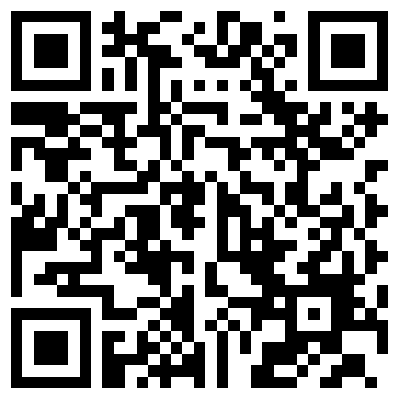
\includegraphics[width=0.5\textwidth]{qr/tb_besprechung_checkout}

\vspace{1cm}
\raggedright
Den Checkout von Proband*innen von Nutzerstudien übernehmen die jeweiligen Versuchsleiter*innen.

\vspace{5mm}
\centering
\huge
\textbf{Diese Registrierung ist verpflichtend! \\ Wird sie nicht durchgeführt, so können Sie von der Labornutzung ausgeschlossen werden!}

\end{document}
